\section*{Problem 4}
\begin{enumerate}
\item See the attached R code for the data normalization and splits.
\item We applied the best subset selection on the training set. Figure 1 shows the curves for $R^2$, adjusted $R^2$, $C_p$ and BIC as a function of the number of predictors. As expected $R^2$ increases as the number of predictors increases. During training we try to estimate the model coefficients such that the RSS is as small as possible, and adding more predictors means the training error will get smaller. However, this does not mean the test error will get smaller. Since our real goal is to reduce test error, RSS and $R^2$ are not good measures of a "best" model. Adjusted $R^2$ and $C_p$ both suggest that models with 7 predictors would be the best model, since these models have the highest adjusted $R^2$ and lowest $C_p$. These two also show that a model with 6 predictors will achieve about the same performance. BIC replaces the penalty term used by $C_P$ ,$2d\hat{\sigma}^2$, with $log(n)d\hat{\sigma}^2$, where $n$ is the number of observations. Since $log(n) > 2$ for any $n >7$, BIC places a heavier penalty of models with more predictors. This can be observed in Figure 1, where the BIC statistic suggests a model with 2-4 predictors is best. Which model should we choose, a model with 6-7 predictors as indicated by the $C_P$ statistic (and corroborated by the $R^2$ statistic, even though it's not a well motivated in statistical theory as the other statistics), or a model with 2-4 predictors as indicated by the BIC statistic? We'll choose the simplest "best" model, which is two predictor model indicated by the BIC statistic. Figure 2 shows the the selected features used for the best model for the range of predictors. In our selected model the features used are \textit{lcavol} and \textit{lweight}.  The \textbf{training error} for this model is 0.553. The \textbf{test error} is []. 
\newline
\begin{figure}[htbp]
\centering
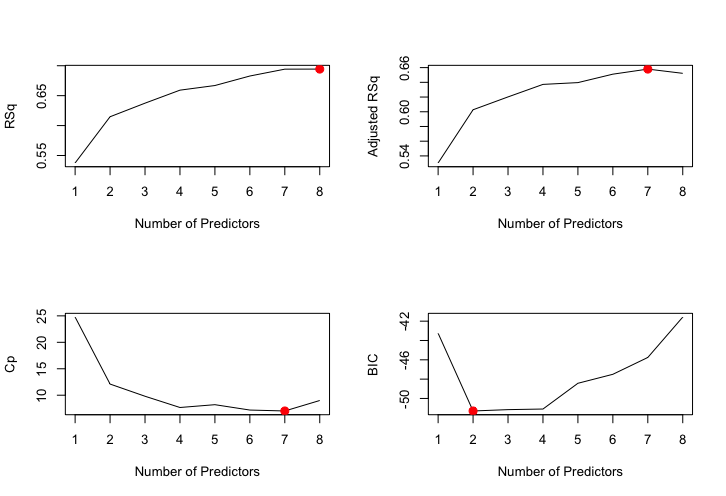
\includegraphics[scale=0.7]{Best_subset.png}
\caption{RSq, adjusted RSq, Cp and BIC values versus the number of predictors in best subset selection.}
\end{figure}
\newline
\begin{figure}[htbp]
\centering
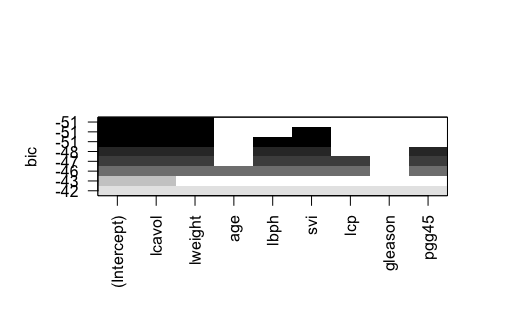
\includegraphics[scale=0.7]{Features.png}
\caption{Selected features for best model with predictors from BIC statistic.}
\end{figure}
\item Figure 3 shows the results of the ridge regression fit on the training data, specifically the values of the coefficients in relation to $\lambda$. The results are as expected. On the left hand side $\lambda$ is almost zero, therefore the ridge coefficient estimates are essentially the same as the least squares estimates. As $lambda$ increases the coefficient estimates shrink to zero. On the right hand side of the plot, when $lambda$ is large, all of the estimates are zero.
\newline
\begin{figure}[htbp]
\centering
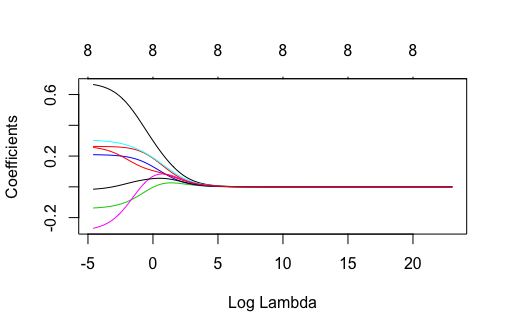
\includegraphics[scale=0.7]{Ridge.png}
\caption{Ridge regression coefficients in relation to $lambda$.}
\end{figure}
\item See code for 5-fold cross-validation for the ridge regression model. For this model the \textbf{training error} in MSE is 0.09645, and the \textbf{test error} is 0.49327. 
\item Figure 4 shows the plot of the lasso coefficient estimates plotted against $\lambda$. As expected, on the far left, when $\lambda$ is zero, the lasso gives the least squares fit, and when $lambda$ is large the coefficient estimates shrink to zero. For the ridge regression the coefficients all smoothly shrink to zero, however for the lasso coefficients most of them sharply shrink to zero as $lambda$ increases.    
\newline 
\begin{figure}[htbp]
\centering
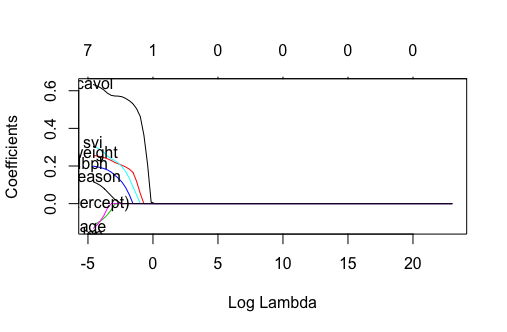
\includegraphics[scale=0.7]{Lasso.png}
\caption{Lasso coefficients in relation to $lambda$.}
\end{figure}
\item See the code for 5-fold cross-validation for the lasso model. For this model the \textbf{training error} is 0.09423, and the \textbf{test error} is 0.45305. [How many features?? Compare coef.]
\item For the linear regression model on all the features the \textbf{training error} is [] and the \textbf{test error} is []. 
\end{enumerate}